\documentclass{article}
\usepackage[english,russian]{babel}
\usepackage{textcomp}
\usepackage{geometry}
  \geometry{left=2cm}
  \geometry{right=1.5cm}
  \geometry{top=1.5cm}
  \geometry{bottom=2cm}
\usepackage{tikz}
\usepackage{multicol}
\usepackage{hyperref}
\usepackage{amsmath}
\usepackage{listings}
%\setlength{\parindent}{0pt}
\pagenumbering{gobble}

\lstset{
  language=C,
  basicstyle=\linespread{1.1}\ttfamily,
  columns=fixed,
  basewidth=0.5em,
  keywordstyle=\color{blue}\bfseries,
  commentstyle=\color{gray},
  texcl=true,
  escapechar =`,
  escapebegin=\lst@commentstyle,
  stringstyle=\ttfamily\color{orange!50!black},
  showstringspaces=false,
  backgroundcolor=\color{white},
  breaklines=true,
  breakatwhitespace=true,
  xleftmargin=5mm,
  keepspaces = true,
  extendedchars=\true,
  tabsize=4,
  upquote=true,
}


\begin{document}




\title{Семинар \#1: Основы C. Ввод/вывод. Операторы. Циклы. Массивы. \vspace{-5ex}}\date{}\maketitle
\section*{Почему C?}
\begin{itemize}
\item \textbf{Язык C это возможно самый влиятельный язык в истории программирования}\\
Он появился в 1972 году и повлиял на многие языки, который появились после него, такие как C++, C\#, Java и многие другие. После изучения C, вам будет проще изучать другие языки.

\item \textbf{Язык C популярный}\\
Несмотря на "старость", язык C сейчас является одним из самых популярных языков программирования.
Многие проекты, в том числе новые, до сих пор пишутся на языке C.

\item \textbf{Язык C компактный}\\
Он содержит в себе относительно немного языковых конструкций и большую часть синтаксиса языка вполне можно 
изучить меньше чем за один семестр.

\item \textbf{Язык C быстрый}\\
Язык позволяет писать код, который будет работать так быстро, насколько это возможно.
На других языках сложно написать код, который будет так же быстр, как код на языках C и C++.


\item \textbf{Язык C является основой для языка C++}\\
C++ был создан на основе языка, поэтому первый шаг для полноценного изучения языка C++ это изучение языка C.
Несмотря на это, это разные языки. В язык C++ было добавлено так много новых возможностей по сравнению с C,
что код на C++ обычно выглядит совершенно по другому.
C++ это гораздо более сложный язык, требующий для изучения хорошего знания C.
\end{itemize}


\section*{Функция \texttt{main}}
\indent Любая программа на языке C должна содержать функцию \texttt{main}.
Эта функция является точкой входа в программу, с неё программа начинает своё выполнение.
Тему \textit{"Функции"} мы будем проходить через несколько занятий.
На данный момент единственное, что вы должны знать, это то что весь код нужно писать внутри фигурных скобочек \texttt{{}} у функции \texttt{main}.
Вот простейшая программа на языке C: 
\begin{lstlisting}
int main() {}
\end{lstlisting}
Она ничего не делает, так как внутри фигурных скобочек \texttt{\{\}} ничего нет.


\section*{Комментарии}
Комментарии в языках программирования -- это поясняющий текст в исходном коде, который игнорируется компилятором. В языке C однострочные комментарии начинаются с \texttt{//}, а многострочные начинаются с \texttt{/*} и заканчиваются на \texttt{*/}.
\begin{lstlisting}
int main() 
{
    // ~ Это однострочный комментарий
    
    /*
    	`Это`
    	`Многострочный`
    	`Комментарий`
    */
}
\end{lstlisting}




\section*{Печать на экран. Функция \texttt{printf}.}
\subsection*{Программа Hello World!}
Давайте рассмотрим простейшую программу, которая хоть что-то делает. Данная программа выводит на экран (то есть в терминал) строку \texttt{Hello World!}. Чтобы это сделать мы используем функцию \texttt{printf} из библиотеки \texttt{stdio.h}. Эта функция принимает строку (выражение в кавычках "{}"{} называется строкой) и печатает её на экран. Для подключения необходимой библиотеки \texttt{stdio.h} используем директиву \texttt{\#include}.
\begin{lstlisting}
#include <stdio.h>
int main() 
{
    printf("Hello World!\n");
}
\end{lstlisting}


\subsection*{Функция \texttt{printf}}
\texttt{printf} это сокращение от \textit{print formatted}, что переводится как форматированная печать.
Печать форматированная, потому что с помощью этой функции можно печатать какие-либо объекты в разных форматах.
Например, если мы в будущем захотим напечатать с помощью \texttt{printf} вещественное число, то можно будет
указать количество знаков после запятой и другие параметры. Функция \texttt{printf} не является встроенной в язык C, она содержится в библиотеки \texttt{stdio.h}, чтобы функция \texttt{printf} работала корректно, нужно обязательно подключать эту библиотеку.

\subsection*{Особые символы}
Для печати особых символов в функции \texttt{printf} используются экранирующие последовательности, которые начинаются с обратного слэша \texttt{"\textbackslash"}.
\\[0.5em]
\texttt{
\begin{tabular}{ l | l }
\texttt{\textbackslash n}	& перенос на новую строку (аналог нажатию \texttt{Enter} в текстовом редакторе) \\ 
\texttt{\textbackslash t} 	& табуляция (аналог нажатию \texttt{Tab} в текстовом редакторе) \\
\texttt{\textbackslash \textbackslash} 	& один символ обратного слэша (\texttt{\textbackslash}) \\ 
\end{tabular}
}
\\[0.5em]
\noindent Например, такая программа:
\begin{lstlisting}
#include <stdio.h>
int main() 
{
    printf("One\n\tTwo\n\t\tThree\n");
}
\end{lstlisting}
Напечатает на экран следующее:
\begin{verbatim}
One
    Two
        Three
\end{verbatim}
Тут, правда, нужно уточнить, что ширина табуляции в разных приложениях может различаться. В примере выше используется табуляция шириной в 4 пробела. В других приложениях ширина табуляции может быть 2 пробела или 8 пробелов.


\section*{Целочисленные переменные \texttt{int}}
\textit{Переменная в C} -- это именованная область памяти компьютера, которая используется для хранения данных.
Её значение может изменяться во время выполнения программы.

Переменные могут иметь разный тип. Разные типы переменных хранят разные виды данных. Переменные одного типа могут хранить целые числа, а переменные другого типа могут хранить дробные числа или строки.
Переменные типа \texttt{int} предназначены для хранения целых чисел (как положительных так и отрицательных).
\texttt{int} это сокращение от слова \textit{integer}, что в переводе означает целое число.


\subsection*{Объявление переменных}
В отличии от многих высокоуровневых языков программирования (таких, как Python), в языке C вы не можете сразу использовать переменную. Прежде чем использовать переменную, вам нужно её объявить. Для объявления переменных используется следующий синтаксис:
\begin{verbatim}
   тип_переменной имя_переменной;
\end{verbatim}
Например, чтобы объявить переменную типа \texttt{int} под названием \texttt{cat}, нужно написать:
\begin{lstlisting}
int cat;
\end{lstlisting}

\subsection*{Инициализация переменных}
Инициализация переменной, это присвоение переменной её начального значения. Инициализацию можно провести вместе с объявлением или после объявления.
\begin{lstlisting}
int cat = 10;	// ~Объявление и инициализация
int dog;		// ~Сначала объявили
dog = 20;       // ~Потом инициализируем
\end{lstlisting}

\subsection*{Печать значений переменных, с помощью функции \texttt{printf}}
Для вывода значений переменных на экран используется функция \texttt{printf}.
Для этого в первом аргументе этой функции -- строке форматирования -- указывают, где именно должно появиться значение переменной. Например, чтобы вывести число типа \texttt{int}, в нужном месте строки пишут \texttt{\%i}. Тогда вместо  \texttt{\%i}  подставится значение переменной. \texttt{\%i} и другие подобные включения в строку форматирования называются \textit{спецификаторами}.
\begin{lstlisting}
#include <stdio.h>
int main()
{
    int age = 10;
    printf("I am %i years old\n", age);
}
\end{lstlisting}
Эта программа напечатает на экран:
\begin{verbatim}
   I am 10 years old
\end{verbatim}
Для печати нескольких значений, можно использовать несколько спецификаторов \texttt{\%i}:
\begin{lstlisting}
#include <stdio.h>
int main()
{
    int age = 10;
    int n = 20;
    printf("I'm %i now, I'll be %i tomorrow. I have %i friends\n", age, age + 1, n);
}
\end{lstlisting}
Эта программа напечатает на экран:
\begin{verbatim}
   I'm 10 now, I'll be 11 tomorrow. I have 20 friends.
\end{verbatim}
Для того, чтобы напечатать на экран одно число, просто уберите из строки форматирования лишние слова:
\begin{lstlisting}
#include <stdio.h>
int main()
{
    int a = 10;
    int b = 20;
    printf("%i\n", a + b); //~ Напечатает 30
}
\end{lstlisting}


\subsection*{Печать числа с фиксированной шириной поля}
В строке форматирования можно задать минимальное число символов, которые будут использованы для печати числа. Например, чтобы ширина поля была минимум 3 символа нужно использовать спецификатор \texttt{\%3i} вместо \texttt{\%i}.
Если число окажется меньше, то \texttt{printf} добавит необходимое количество пробелов перед числом. Если печатаемое число занимает больше символов, чем заданная ширина поля, то оно напечатается полностью.
\begin{lstlisting}
#include <stdio.h>
int main()
{
    printf("%3i\n", 1);
    printf("%3i\n", 12);
    printf("%3i\n", 123);
}
\end{lstlisting}
Данная программ напечатает:
\begin{verbatim}
     1
    12
   123
\end{verbatim}
Если использовать спецификатор \texttt{\%03i}, то вместо пробелов будут использоваться нули.
\begin{lstlisting}
#include <stdio.h>
int main()
{
    printf("%03i\n", 1);
    printf("%03i\n", 12);
    printf("%03i\n", 123);
}
\end{lstlisting}
Данная программ напечатает:
\begin{verbatim}
   001
   012
   123
\end{verbatim}
Данный формат печати удобен, если вам нужно красиво напечатать таблицу чисел. Без такого форматирования числа будут "съезжать"{}, так как разные числа будут занимать разное количество символов. Ещё один случай, когда такая печать может понадобиться, это печать некоторых форматов, например времени:
\begin{lstlisting}
#include <stdio.h>
int main()
{
	int h = 12;
	int m = 30;
	printf("%02i:%02i\n", h, m);  //~ напечатает 12:30
	
	h = 9;
	m = 5;
	printf("%02i:%02i\n", h, m);  //~ напечатает 09:05
}
\end{lstlisting}


\newpage
\section*{Адрес и размер переменной}
\subsection*{Переменные в памяти}
\begin{itemize}
\item 1 бит -- минимальная единица измерения памяти. В 1 бите может хранится либо \texttt{0} либо \texttt{1}.
\item Вся память делится на ячейки, размером в 8 бит = 1 байт.
\item Все эти ячейки (байты) занумерованы, номер ячейки называется адресом. Байт -- это минимальная адресуемая единица памяти.
\item Переменные размещаются в памяти непрерывными блоками. Размер любой переменной составляет целое число байтов (не менее 1).
\item У любой переменной можно получить её адрес. Адрес переменной -- это адрес первого байта переменной.
\item Чтобы найти адрес переменной, нужно перед ней поставить \texttt{\&}, например, \texttt{\&a}.
\item Чтобы найти размер переменной в байтах: \texttt{sizeof(a)}.
\item Переменная типа \texttt{int} \textit{обычно} имеют размер 4 байта = 32 бита. Значит в ней может хранится максимум $2^{32}$ значений. То есть переменные типа \texttt{int} могут принимать значения от $-2^{31}$ до $2^{31} - 1$.
\end{itemize}



\subsection*{Расположение переменных типа \texttt{int} в памяти}
На большинстве систем переменные типа \texttt{int} занимают 4 байта. Соответственно, если вы создадите 3 переменные типа \texttt{int} вот так:
\begin{lstlisting}
int a = 10;
int b = 20;
int c = 30;
\end{lstlisting}
то в памяти это может выглядеть вот так (на самом деле чуть сложнее, но это мы разберём в дальнейшем):
\begin{center}
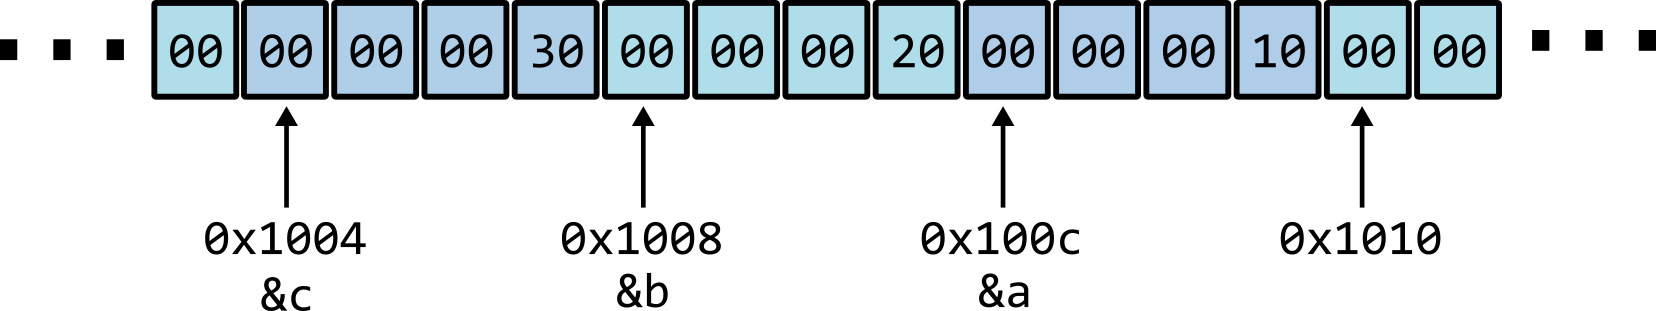
\includegraphics[scale=1]{../images/memory2.png}
\end{center}
Адрес переменной -- это адрес первого байта того участка памяти, который занимает данная переменная.
Чтобы получить адрес переменной в языке C нужно написать перед именем переменной символ \texttt{\&}.
Для печати адреса с помощью \texttt{printf} используется спецификатор \texttt{\%p}. 
В этом случае адрес напечатается в шестнадцатеричной системе счисления.
\begin{lstlisting}
#include <stdio.h>
int main()
{
    int a = 10;
    int b = 20;
    printf("Address of a = %p\n", &a);    	//~ Печатаем адрес переменной a
    printf("Address of b = %p\n", &b);    	//~ Печатаем адрес переменной b
    printf("Size of a = %zu\n", sizeof(a));	//~ Печатаем размер переменной a
    printf("Size of b = %zu\n", sizeof(b));	//~ Печатаем размер переменной a
}
\end{lstlisting}
Важно отметить, что адреса переменных могут быть разными при разных запусках программы. Операционная система рандомизируют адресное пространство для безопасности и гибкости.


\section*{Считывание переменных. Функция \texttt{scanf}.}
\textit{Считывание} — процесс получения данных из внешнего источника (клавиатура, файлы) и сохранения их в переменные.
Для ввода данных с клавиатуры используется функция \texttt{scanf} из библиотеки \texttt{stdio.h}. При достижении этой функции выполнение программы приостанавливается до ввода пользователем данных. Данные нужно ввести в экран терминала. После ввода данные сохраняются в указанные переменные.
\subsection*{Считывание переменных типа \texttt{int}}
Для того, чтобы считать значение переменной \texttt{a} нужно написать:
\begin{lstlisting}
scanf("%i", &a);
\end{lstlisting}
\textbf{Важно!} Обратите внимание, что функции \texttt{scanf} нужно передавать именно \textit{адрес переменной}, а не само значение переменной. В отличии от функции \texttt{printf}, куда нужно передавать саму переменную
И это логично, ведь функции \texttt{printf} для печати нужно само значение переменной.
А функции \texttt{scanf} текущее значение переменной не нужно, ей нужен только адрес того места, куда надо записать новое, считанное с экрана значение.\\
\noindent Приведём пример, простой программы, которая считывает число и печатает это число, увеличенное в 2 раза.
\begin{lstlisting}
#include <stdio.h>
int main()
{
    int a;
    scanf("%i", &a);
    printf("%i\n", 2 * a);
}
\end{lstlisting}

\subsection*{Считывание нескольких переменных типа \texttt{int}}
Можно считать несколько переменных, используя лишь один вызов функции \texttt{scanf}. В следующей программе считываются 2 числа и печатается из сумма.
\begin{lstlisting}
#include <stdio.h>
int main()
{
    int a;
    int b;
    scanf("%i%i", &a, &b);
    printf("%i\n", a + b);
}
\end{lstlisting}

\subsection*{Форматированное считывание}
Форматирование можно использовать не только у функции \texttt{printf}, но и у функции \texttt{scanf}.
Рассмотрим, например, следующую программу:
\begin{lstlisting}
#include <stdio.h>
int main()
{
    int a;
    int b;
    scanf("(%i,%i)", &a, &b);
    printf("%i\n", a + b);
}
\end{lstlisting}
Если мы на вход этой программе передадим \texttt{(10,20)}, то \texttt{scanf} корректно распарсит эту строку и запишет в переменную \texttt{a} значение \texttt{10}, а в переменную \texttt{b} -- значение \texttt{20}. Однако, если вы введёте числа в неверном формате, то \texttt{scanf} вернёт ошибку.

\noindent Приведём ещё один пример программы, которая работает с форматированным вводом. Пусть на вход подаются 2 времени в формате \texttt{hh:mm}. Данная программа считывает эти времена, корректно складывает их и печатает в таком же формате.
\begin{lstlisting}
#include <stdio.h>
int main()
{
    int h1, m1;
    scanf("%i:%i", &h1, &m1);
    int h2, m2;
    scanf("%i:%i", &h2, &m2);

    int total_minutes = 60 * h1 + m1 + 60 * h2 + m2;
    int h = total_minutes / 60;
    int m = total_minutes % 60;
    printf("%02i:%02i\n", h, m);
}
\end{lstlisting}
Если теперь на вход данной программе мы передадим
\begin{verbatim}
   02:40 
   06:25
\end{verbatim}
то программа напечатает
\begin{verbatim}
   09:05
\end{verbatim}

\subsection*{Функция \texttt{scanf} и пробельные символы}
Пробельные символы играют важную роль при работе с функцией \texttt{scanf}. К пробельным символам относятся:
\begin{itemize}
\item Пробел (\texttt{{}"{} {}"{}})
\item Табуляция  (\texttt{"\textbackslash t"})
\item Перевод строки  (\texttt{"\textbackslash n"})
\item Другие пустые символы
\end{itemize}
Дело в том, что функция \texttt{scanf} часто "съедает"{} эти символы. Чтобы правильно её использовать, важно понимать, когда именно это происходит. Запомните два правила:
\begin{itemize}
\item Если \texttt{scanf} встречает в строке форматирования пробельный символ (или несколько подряд), она будет считывать все пробелы, табуляции и переводы строк до тех пор, пока не наткнётся на первый непробельный символ. При этом количество и тип пробелов в форматной строке и во вводе могут не совпадать.

\item Если \texttt{scanf} встречает спецификатор для считывания числа (например, \texttt{\%i}), она также пропускает все пробельные символы до первого непробельного, и только потом начинает считывать число.
\end{itemize}
 
Например, если написать:
\begin{lstlisting}
scanf("%i", &a);
\end{lstlisting}
и перед числом ввести в терминале пробелы, табуляции или переводы строк, то число всё равно будет корректно считано. Если использовать:
\begin{lstlisting}
scanf("%i%i", &a, &b);
\end{lstlisting}
то пробельные символы можно ставить как перед первым числом, так и между числами -- ввод всё равно будет обработан правильно. А запись:
\begin{lstlisting}
scanf("%i    %i", &a, &b);
\end{lstlisting}
работает аналогично: при вводе разрешено любое количество пробелов или других пробельных символов между числами.


\subsection*{Некорректное использование \texttt{scanf} при считывании чисел}
Одной из самых распространённых ошибок при использовании \texttt{scanf} демонстрируется в следующей программе:
\begin{lstlisting}
#include <stdio.h>
int main()
{
    int a;
    scanf("%i\n", &a);
    printf("%i\n", a * a);
}
\end{lstlisting}
Эта программа должна была считывать число и печатать его квадрат, но программа почему-то работает не так как надо. Вместо того, чтобы просить одно число программа почему-то просит два числа. Но затем правильно печатает квадрат первого введённого числа.

\noindent Ошибка заключается в том, что в строке форматирования \texttt{scanf} содержится лишний пробельный символ \texttt{\textbackslash n}:
\begin{lstlisting}[literate={\\n}{{\textcolor{red}{\textbackslash n}}}2]
scanf("%i\n", &a);
\end{lstlisting}
А как было сказано выше, как только \texttt{scanf} увидит любой пробельный символ в строке форматирования, он будет считывать все пробельные символы, пока не встретит первый непробельный.


\newpage
\section*{Операторы}
\subsection*{Арифметические операторы}
К целочисленным переменным, таким как переменные типа \texttt{int} можно применять арифметические операции, используя следующие операторы:
\begin{center}
\texttt{
\begin{tabular}{ c c } 
 + & сложение \\  
 - & вычитание \\  
 * & умножение \\ 
 / & целочисленное деление \\
 \% & остаток \\
\end{tabular}
}
\end{center}

\noindent Приведём пример программы, использующей эти операторы.
\begin{lstlisting}
#include <stdio.h>
int main()
{
    int a = 17;
    int b = 7;
    
    printf("%i\n", a + b); //~ напечатает 24
    printf("%i\n", a - b); //~ напечатает 10
    printf("%i\n", a * b); //~ напечатает 119
    printf("%i\n", a / b); //~ напечатает 2 (так 17 / 7 = 2 (3 в остатке))
    printf("%i\n", a % b); //~ напечатает 3 (так 17 / 7 = 2 (3 в остатке))
}
\end{lstlisting}
Если вы никогда не программировали, принцип целочисленного деления может показаться неочевидным. Поскольку тип \texttt{int} предназначен для целых чисел, результат любой операции между ними также будет целым числом. Поэтому при делении дробная часть просто отбрасывается.

\subsection*{Примеры использования оператора остатка \texttt{\%}}
Приведём примеры использования оператора остатка. 
\begin{itemize}
\item Программа, которая считывает число и печатает последнюю цифру числа в десятичной записи:
\begin{lstlisting}
#include <stdio.h>

int main()
{
	int a;
	scanf("%i", &a);
	printf("%i\n", a % 10);
}
\end{lstlisting}

\item Программа, которая считывает число и печатает \texttt{0}, если число чётное и \texttt{1}, если нечётное:
\begin{lstlisting}
#include <stdio.h>

int main()
{
	int a;
	scanf("%i", &a);
	printf("%i\n", a % 2);
}
\end{lstlisting}
\end{itemize}

\subsection*{Оператор присваивания}
Оператор присваивания(\texttt{=}) используется для присвоения значений переменным. Также, как и другие бинарные операторы он требует двух операндов. Но в отличии от арифметических операторов он изменяет значение одного из своих операндов, а именно, после присваивания значение левого операнда изменится и станет равно значению правого операнда.
\begin{lstlisting}
#include <stdio.h>
int main()
{
	int a;				//~ Объявляем переменную
	a = 10;             //~ Задаём значение, используя оператор присваивания =
	printf("%i\n", a);  //~ Напечатает 10
}
\end{lstlisting}

\noindent Следует отличать оператор присваивания от инициализации при объявлении переменной. 
\begin{lstlisting}
#include <stdio.h>
int main()
{
	int a = 10;			//~ Объявляем и инициализируем переменную
		    			//~ Тут оператор присваивания не используется
	
	printf("%i\n", a);  //~ Напечатает 10
}
\end{lstlisting}
Несмотря на использование одинакового символа \texttt{=} и схожего конечного результата, инициализация при объявлении и операция присваивания фундаментально различаются на семантическом уровне. Для компилятора это различные операции, выполняемые на разных этапах работы с переменной.

\subsection*{Возвращаемое значение оператора присваивания}
Оператор присваивания не только изменяет значение левого операнда. Он также, как и все другие операторы, возвращает значение. А именно, он возвращает новое значение левого операнда.
\begin{lstlisting}
#include <stdio.h>

int main()
{
    int a = 10;
    int b = 20;
    printf("%i\n", a = b);  //~ Напечатает 20
}
\end{lstlisting}


\subsection*{Составные операторы присваивания}
Помимо обычного оператора присваивания существуют составные операторы, которые объединяют арифметическую операцию с операцией присваивания.
\begin{center}
\texttt{
\begin{tabular}{ l l l}
 = & оператор присваивания & присвоить левой части правую\\ 
 += & оператор присваивания сложения & прибавить к левой части правую \\  
 -= & оператор присваивания вычитания & отнять от левой части правую \\  
 *= & оператор присваивания умножения & умножить левую часть на правую \\  
 /= & оператор присваивания деления & разделить левую часть на правую \\ 
 \%= & оператор присваивания взятия остатка & левая часть становится равна остатку\\
\end{tabular}
}
\end{center}
Также как обычный оператор присваивания, все эти операторы возвращают новое значение левого операнда.



\subsection*{Операторы инкремента и декремента}
Операторы инкремента и декремента увеличивают или уменьшают значение переменной на 1. 
\begin{center}
\texttt{
\begin{tabular}{ l l l}
 ++ &  & увеличить на 1\\
 -{}- &  & уменьшить на 1
\end{tabular}
}
\end{center}

\noindent Это унарные операторы, то есть они применяются только к одно переменной. Различают префиксные операторы инкремента (пишутся перед переменной) и постфиксные (пишутся после переменной).
\begin{lstlisting}
#include <stdio.h>
int main()
{
    int a = 10;
    ++a;				//~ Префиксный инкремент
    a++;				//~ Постфиксный инкремент
    printf("%i\n", a);	//~ Напечатает 12
}
\end{lstlisting}

\subsection*{Возвращаемое значение операторов инкремента и декремента}
Префиксный и постфиксный операторы инкремента и декремента различаются возвращаемым значением.
\begin{itemize}
\item Префиксный (\texttt{++a}) возвращает новое значение.
\item Постфиксный (\texttt{a++}) возвращает старое значение.
\end{itemize}
\begin{lstlisting}
#include <stdio.h>
int main()
{
    int a = 10;
    int b = 10;
    printf("%i\n", ++a);  //~ Напечатает 11
    printf("%i\n", b++);  //~ Напечатает 10
    printf("%i\n", a);    //~ Напечатает 11
    printf("%i\n", b);    //~ Напечатает 11
}
\end{lstlisting}

\subsection*{Операторы сравнения}
Операторы сравнения в языке C всегда возвращают целые числа типа \texttt{int}.
\begin{center}
\texttt{
\begin{tabular}{ l | l}
 оператор    		& возвращаемое значение\\ \hline
 a == b				& 1 если равны, иначе 0\\ 
 a != b  			& 1 если не равны, иначе 0\\  
 a > b   			& 1 если больше, иначе 0\\  
 a >= b  		 	& 1 если больше или равно, иначе 0\\ 
 a < b   			& 1 если меньше, иначе 0\\
 a <= b   		 	& 1 если меньше или равно, иначе 0\\
\end{tabular}
}
\end{center}

\begin{lstlisting}
#include <stdio.h>
int main()
{
    int a = 10;
    int b = 20;
    printf("%i\n", a < b);	//~ Напечатает 1
    printf("%i\n", a == b);	//~ Напечатает 0
}
\end{lstlisting}


\subsection*{Булевая алгебра}
В булевой алгебре есть два элемента $0$ и $1$. Часто эти элементы также называют \textit{false} (ложь) и \textit{true} (истина). Также в булевой алгебре есть 3 основные операции:

\begin{itemize}
\item \textbf{Логическое И} -- истинно только тогда, когда оба операнда истинны.
\begin{verbatim}
                0 И 0 = 0
                0 И 1 = 0
                1 И 0 = 0
                1 И 1 = 1
\end{verbatim}

\item \textbf{Логическое ИЛИ} -- истинно только тогда, когда хотя бы один из операндов истинен.
\begin{verbatim}
                0 ИЛИ 0 = 0
                0 ИЛИ 1 = 1
                1 ИЛИ 0 = 1
                1 ИЛИ 1 = 1
\end{verbatim}

\item \textbf{Логическое НЕ} -- инвертирует значение операнда.
\begin{verbatim}
                НЕ 0 = 1
                НЕ 1 = 0
\end{verbatim}
\end{itemize}


\subsection*{Логические операторы}
В языке C в логические операторы обозначаются следующим образом:
\begin{center}
\texttt{
\begin{tabular}{ c c }
 \&\& & логическое И \\ 
 || & логическое ИЛИ \\  
 !  & логическое НЕ \\  
\end{tabular}
}
\end{center}
Операнды логических операторов в языке C -- это целые числа. При этом они интерпретируются так:
\begin{itemize}
\item Число, равное нулю -- воспринимается как элемент $0$ (ложь).
\item Любое число, отличное от нуля -- воспринимается как элемент $1$ (истина).
\end{itemize}
Все логические операторы возвращают \texttt{0} или \texttt{1} -- целое число типа \texttt{int}.\\
Пример программы, которая печатает возвращаемые значения логических операторов:
\begin{lstlisting}
#include <stdio.h>
int main()
{
    int a = 10;
    int b = 0;
    printf("%i\n", a && b);		//~ Напечатает 0
    printf("%i\n", a || b);		//~ Напечатает 1
    printf("%i\n", !a);			//~ Напечатает 0
}
\end{lstlisting}

\noindent Пример программы, которая использует логические операторы, совместно с другими операторами:
\begin{lstlisting}
#include <stdio.h>
int main()
{
    int a = 10;
    int b = 20;
    printf("%i\n", (a < b) && !(a % 2)); 		//~ Напечатает 1, так как a чётное и меньше b 
    printf("%i\n", (a < b) + (a && b) + !!a);	//~ Напечатает 3
}
\end{lstlisting}


\subsection*{Приоритет операторов}
Таблица содержит все операторы языка C и уровень их приоритета от наиболее к наименее приоритетным.
\begin{center}
\texttt{
\begin{tabular}{ l | l | l}
 приоритет    		& операторы		& описание\\ \hline
 1					& \texttt{++} \texttt{-{}-} 		& постфиксный инкремент/декремент \\ 
   					& \texttt{()}						& оператор вызова функции\\  
   					& \texttt{[]}						& оператор индексирования\\  
   					& \texttt{.} \texttt{->}			& оператор точка и стрелочка\\ \hline  
 2					& \texttt{++} \texttt{-{}-} 		& префиксный инкремент/декремент \\ 
 					& \texttt{+} \texttt{-} 			& унарный плюс и минус \\ 
 					& \texttt{!} \texttt{$\sim$} 		& логическое НЕ и побитовое НЕ \\ 
 					& \texttt{(тип)} 			 		& оператор приведения к типу \\ 
 					& \texttt{*} 			 			& разыменование указателя \\ 
 					& \texttt{\&} 			 			& оператор получения адреса \\ 
 					& \texttt{sizeof} 			 		& оператор получения размера \\ 
 					& \texttt{alignof} 			 		& оператор получения выравнивания \\ \hline  
 3					& \texttt{*} \texttt{/} \texttt{\%} & умножение, деление, остаток \\ \hline  
 4					& \texttt{+} \texttt{-} 			& сложение и вычитание \\ \hline  
 5					& \texttt{<{}<} \texttt{>{}>} 		& побитовый сдвиг влево и вправо \\ \hline  
 6				    & \texttt{<} \texttt{<=} \texttt{>} \texttt{>=} & операторы сравнения \\ \hline  
 7				    & \texttt{==} \texttt{!=} 		 	& операторы сравнения на равенство/неравенство \\ \hline  
 8				    & \texttt{\&}  		 				& побитовое И \\ \hline  
 9				    & \texttt{\^{}}  		 			& побитовое исключающее ИЛИ \\ \hline  
 10				    & \texttt{|}  		 				& побитовое ИЛИ \\ \hline  
 11				    & \texttt{\&\&}  		 			& логическое И \\ \hline  
 12				    & \texttt{||}  		 				& логическое ИЛИ \\ \hline  
 13				    & \texttt{?:}  		 				& тернарный оператор \\ \hline 
 14				    & \texttt{=}  		 				& присваивание \\
  				    & \texttt{+=} \texttt{-=} \texttt{*=} \texttt{/=} \texttt{\%=}  & составные присваивания \\
  				    & \texttt{>{}>=} \texttt{<{}<=} \texttt{\&=} \texttt{\^{}=} \texttt{|=}  & составные побитовые присваивания \\\hline  
 15				    & \texttt{,}  		 				& оператор запятая
\end{tabular} 
}
\end{center}
Эта таблица поможет понять вам в каком порядке вычисляется выражение. Например, в следующем выражении:
\begin{lstlisting}
d = a + b * c;
\end{lstlisting}
сначала выполнится умножение, затем сложение и в конце присваивание. Если нужно изменить порядок вычислений, можно использовать скобки:
\begin{lstlisting}
d = (a + b) * c;
\end{lstlisting}
в таком случае сначала выполнится сложение, потом умножение и в конце присваивание.

\subsection*{Ассоциативность операторов}
Ассоциативность определяет, в каком порядке выполняются операторы с одинаковым приоритетом (слева направо или справа налево).
В C операторы делятся на два типа по ассоциативности:
\begin{itemize}
\item Лево-ассоциативные -- вычисляются слева направо.
\begin{lstlisting}
a - b - c - d      вычисляется как     ((a - b) - c) - d 
\end{lstlisting}
\item Право-ассоциативные -- вычисляются справа налево.
\begin{lstlisting}
a = b = c = d      вычисляется как     a = (b = (c = d))
\end{lstlisting}
\end{itemize}


\newpage

\section*{Инструкции}
\subsection*{Определение понятия "литерал"{}}
\textit{Литерал} -- это непосредственно записанное в коде фиксированное значение, которое используется в программе "как есть"{}, а не вычисляется во время выполнения. Например, в строках:
\begin{lstlisting}
int a = 10;
printf("Hello\n");
\end{lstlisting}
Число \texttt{10} является целочисленным литералом, а строка \texttt{"Hello\textbackslash n"} -- строковым литералом.

\subsection*{Определение понятия "выражение"{} в C}
\textit{Выражение} (англ. \textit{expression}) -- это последовательность операторов и их операндов, задающих некоторое вычисление. В качестве операндов могут служить имена переменных, имена функций и литералы. Обратите внимание, что вызов функции это тоже оператор (оператор круглые скобочки). Примерами выражений могут быть:
\begin{lstlisting}
a + b - 10 / c
printf("Hello\n")
a = 20
a  	//~ Простейшее выражение, состоящее из одной имени переменной
10  //~ Простейшее выражение, состоящее из одного литерала
\end{lstlisting}


\subsection*{Определение понятия "объявление"{} в C}
\textit{Объявление} (англ. \textit{declaration}) -- это конструкция языка, которая добавляет ещё одно имя (идентификатор) в программу и задаёт некоторые свойства этого имени, например такие как тип и начальное значение переменной.
\begin{lstlisting}
int a;
int b = 10;
\end{lstlisting}

\subsection*{Определение понятия "инструкция"{} в C}
\textit{Инструкция} (англ. \textit{statement}) -- это отдельная команда, которую компилятор воспринимает как законченное действие. Инструкции можно разделить на следующие категории:
\begin{itemize}
\item \textit{Пустая инструкция.} Ничего не делает.
\begin{lstlisting}
;
\end{lstlisting}

\item \textit{Инструкции выражения.} Состоит из выражения с точкой с запятой. Просто исполняет это выражение.
\begin{lstlisting}
a + b - 10 / c;
printf("Hello\n");
a = 20;
10;		//~ Простейшая инструкция выражения, состоит из одного литерала. Ничего не делает
a;		//~ Простейшая инструкция выражения, состоит из одного имени. Ничего не делает
\end{lstlisting}

\item \textit{Составная инструкция (блок).} Группа из нуля или более инструкций и/или объявлений, заключенная в фигурные скобки \texttt{\{\}}.
Пример одной составной инструкции:
\begin{lstlisting}
{
	int a = 10;
	int b = 20;
	printf("%i\n", a + b);
}
\end{lstlisting}

\item \textit{Инструкции управления потоком выполнения.} Это инструкции, которые позволяют изменять порядок выполнения программы: переходить по условиям, повторять части кода или завершать работу функции/программы. В эту категорию входят условная инструкция \texttt{if}, инструкции циклов \texttt{for} и \texttt{while} и другие.
\end{itemize}


\subsection*{Блоки и области видимости}
\textit{Блок} -- это составная инструкция, то есть группа из нуля или более инструкций и/или объявлений, заключенная в фигурные скобки.\\
\textit{Область видимости} -- часть программы, где доступно имя переменной или функции.\\
\textit{Блочная область видимости} -- переменные, объявленные внутри блока, доступны только внутри него.
\begin{lstlisting}
#include <stdio.h>
int main() 
{
    int a = 10;
    
    {
        int b = 20;			//~ b не будет видна вне блока, в котором объявлена
        printf("%i\n", a);  //~ ОК, переменная a видна
        printf("%i\n", b);  //~ ОК, переменная b видна
    }

    printf("%i\n", a);  	//~ ОК, переменная a видна
    printf("%i\n", b);  	//~ Ошибка, b вне области видимости
}
\end{lstlisting}

\subsection*{Повторное объявление переменной}
В языке C нельзя объявить две переменных с тем же самым именем в одном и том же блоке. 
\begin{lstlisting}
#include <stdio.h>
int main() 
{
    int a = 10;
    int a = 20;				//~ Ошибка, повторное объявление a
    
    {
        int b = 20;			
        int b = 30;			//~ Ошибка, повторное объявление b
    }
}
\end{lstlisting}


\subsection*{Затенение переменных в блоке}
Если внутри блока объявить переменную с тем же именем, что и внешняя переменная, то внутренняя затенит внешнюю.
\begin{lstlisting}
#include <stdio.h>
int main() 
{
    int a = 10;
    
    {
        printf("%i\n", a);  //~ Видит только внешнюю a. Напечатает 10.
        int a = 20;			//~ Внутренняя переменная a затеняет внешнюю с тем же именем.
        printf("%i\n", a);  //~ Напечатает 20.
    }
    
    printf("%i\n", a);  	//~ Тут внутренняя переменная уже не видна. Напечатает 10.
}
\end{lstlisting}



\newpage
\section*{Инструкции управления потоком выполнения}
\subsection*{Условная инструкция \texttt{if}}
\begin{lstlisting}
                                     if ( условие )
                                         инструкция
\end{lstlisting}
Инструкция \texttt{if} принимает в круглых скобках условие -- выражение, которое вычисляется в целое число. 
\begin{itemize}
\item Если условие не равно \texttt{0}, то следующая после \texttt{if(...)} инструкция исполняется.
\item Если условие равно \texttt{0}, ~~~ то следующая после \texttt{if(...)} инструкция пропускается.
\end{itemize}
Следующая программа напечатает строки \texttt{Cat} и \texttt{Mouse}, но не напечатает \texttt{Dog}:
\begin{lstlisting}
#include <stdio.h>
int main()
{
    if (1)
        printf("Cat\n");

    if (0)
        printf("Dog\n");
        
    if (-10)
        printf("Mouse\n");
}
\end{lstlisting}
Чаще всего инструкция \texttt{if} используется вместе с операторами сравнения:
\begin{lstlisting}
#include <stdio.h>
int main()
{
    int a;
    scanf("%i", &a);

    if (a > 0)
        printf("Positive\n");
}
\end{lstlisting}
Это работает благодаря тому, что операторы сравнения в C возвращают число 1 при истинности условия и 0 при его ложности.\\

\noindent Также часто используются логические операторы:
\begin{lstlisting}
#include <stdio.h>
int main()
{
    int a;
    scanf("%i", &a);

    if (a >= 10 && a < 100)
        printf("Positive two-digit number\n");
        
    if (a < 0 || a % 2)
        printf("Negative or odd number\n");
}
\end{lstlisting}


\subsection*{Инструкция \texttt{if} и блоки}
Нужно помнить, что \texttt{if} "применяется"{} только к одной инструкции, следующий после неё. Например, код:
\begin{lstlisting}
if (a < 0)
    printf("Cat\n");
    printf("Dog\n");
\end{lstlisting}
напечатает строку \texttt{Dog}, даже если переменная \texttt{a} больше нуля, так как к \texttt{if} относится только строка, печатающая \texttt{Cat}. Другими словами, компилятор воспринимает этот код так:
\begin{lstlisting}
if (a < 0)
    printf("Cat\n");
printf("Dog\n");
\end{lstlisting}
Чтобы к \texttt{if} относилось несколько инструкций, нужно объединить эти инструкции с помощью блока:
\begin{lstlisting}
if (a < 0)
{
    printf("Cat\n");
    printf("Dog\n");
}
\end{lstlisting}

\subsection*{Разновидность условной инструкции \texttt{if else}}
\begin{lstlisting}
                                     if ( условие )
                                         инструкция1
                                     else 
                                         инструкция2
\end{lstlisting}
\begin{itemize}
\item Если выражение не равно \texttt{0}, то исполняется инструкция, следующая после \texttt{if(...)}.
\item Если выражение равно \texttt{0}, ~~~ то исполняется инструкция, следующая после \texttt{else}.
\end{itemize}
\begin{lstlisting}
#include <stdio.h>
int main()
{
    int a;
    scanf("%i", &a);
    if (a)
        printf("Non-zero\n");
    else
        printf("Zero\n");
}
\end{lstlisting}
Если нужно объединить несколько зависимых условий, то можно вспомнить, что \texttt{if} и \texttt{if else} сами являются инструкциями, поэтому их можно подставить за место инструкции внутри другого \texttt{if else} так:
\begin{lstlisting}
        if ( условие1 )                                                                             
            инструкция1                                     if ( выражение1 )
        else                                                    инструкция1
            if ( условие2 )                                 else if ( выражение2 )
                инструкция2         что эквивалентно:           инструкция2
            else                                            else if ( выражение3 )            
                if ( условие3 )                                 инструкция3
                    инструкция3                             else
                else                                            инструкция4
                    инструкция4                                                                                                                        
\end{lstlisting}

Приведём пример программы, использующей несколько зависимых условий:
\begin{lstlisting}
#include <stdio.h>
int main() 
{
    int month;
    scanf("%i", &month);
    
    if (month == 12 || month == 1 || month == 2)
    {
        printf("Winter\n");
    }
    else if (month >= 3 && month <= 5) 
    {
        printf("Spring\n");
    }
    else if (month >= 6 && month <= 8) 
    {
        printf("Summer\n");
    }
    else if (month >= 9 && month <= 11) 
    {
        printf("Autumn\n");
    }
    else 
    {
        printf("Error!\n");
    }
}
\end{lstlisting}




\subsection*{Инструкция цикла \texttt{while}}
\begin{lstlisting}
                                     while ( условие )
                                         инструкция
\end{lstlisting}
Также как и \texttt{if}, инструкция \texttt{while} принимает в круглых выражение, которое вычисляется в целое число. Будем называть это выражение условием.
\begin{itemize}
\item Если условие равно \texttt{0}, то следующая после \texttt{while} инструкция не выполняется.
\item Если условие не равно \texttt{0}, то инструкция выполняется. После этого условие снова проверяется, его значение могло измениться за время выполнения инструкции.
Если условие вновь не равно \texttt{0}, то инструкция снова выполняется и снова проверяется условие.
Так продолжается пока условие не станет равным 0.
\end{itemize}
Рассмотрим пример использования цикла \texttt{while}. В этой программе составная инструкция, следующая после \texttt{while} исполнится 5 раз пока значение переменной \texttt{a} не станет равным нулю.
\begin{lstlisting}
#include <stdio.h>
int main()
{
    int a = 5;
    while (a)
    {
        printf("%i\n", a);
        a -= 1;
    }
}
\end{lstlisting}


\subsection*{Бесконечные циклы}
Бесконечный цикл -- это цикл, который выполняются бесконечно, так как их условие никогда не становится равным нулю. Пример программы, содержащей бесконечный цикл:
\begin{lstlisting}
#include <stdio.h>
int main()
{
    while (1)
        printf("Hello\n");
}
\end{lstlisting}
Если такую программу запустить в терминале и не предпринимать никаких дополнительных действий по её завершению, то она будет работать вечно, потребляя ресурсы системы. Для принудительного завершения программы в терминале используйте сочетание клавиш \texttt{Ctrl-C}.

\subsection*{Тело цикла и итерирование}
Чаще всего инструкцией, следующей после \texttt{while} является составная инструкция (блок). То есть цикл \texttt{while} часто выглядит так:
\begin{lstlisting}
                                     while ( условие )
                                     {
                                         инструкция1
                                         инструкция2
                                         ...
                                     }
\end{lstlisting}
Набор инструкций внутри блока, следующего после \texttt{while}, называется \textit{телом цикла}.
Один проход по телу цикла называют \textit{итерацией}, а весь процесс многократных итераций -- \textit{итерированием}.

\subsection*{Итерирование до заданного числа}
Часто требуется произвести итерирование от нуля до некоторого заданного числа. Разберём этот случай на примере следующей программы, которая считывает число $n$, а затем $n$ раз печатает на экран строку \texttt{"Hello"{}}:
\begin{lstlisting}
#include <stdio.h>
int main()
{
	int n;
	scanf("%i", &n);
	int i = 0;
    while (i < n)
    {
        printf("Hello\n");
        i += 1;
    }
}
\end{lstlisting}
Для этой задачи мы завели специальную целочисленную переменную \texttt{i}, чьё назначение заключается в том чтобы проверяться в условии перед каждой итерацией и изменяться в конце каждой итерации. Такая переменная называется \textit{счётчик} (англ. \textit{counter}). Общепринято использовать имя \texttt{i} для таких переменных. Для увеличения счётчика в конце итерации часто используется оператор инкремента:
\begin{lstlisting}
	int i = 0;
    while (i < 5)
    {
        printf("Hello\n");
        i++;
    }
\end{lstlisting}

\subsection*{Считывание \texttt{n} чисел в цикле}
Часто возникает задача обработки последовательности чисел, поступающих на вход. Во многих случаях нет необходимости сохранять все эти числа в массив для последующей обработки (работа с массивами будет рассмотрена несколько позже). Вместо этого можно последовательно считывать каждое число в одну и ту же переменную и немедленно обрабатывать его.

Рассмотрим программу, на вход которой поступает пять чисел, а она печатает эти числа, увеличенные на 1:
\begin{lstlisting}
#include <stdio.h>
int main()
{
    int i = 0;
    while (i < 5)
    {
        int a;
        scanf("%i", &a);
        printf("%i ", a + 1);
        ++i;
    }
    printf("\n");
}
\end{lstlisting}
Если на вход этой программе передать:
\begin{verbatim}
10 20 30 40 50
\end{verbatim}
то она напечатает:
\begin{verbatim}
11 21 31 41 51
\end{verbatim}

\noindent Для обработки последовательности чисел произвольной длины, можно первым числом подавать на вход количество элементов в последовательности, а затем уже подавать сами числа. В самой программе мы сначала используем \texttt{scanf} один раз для считывания количества чисел, а затем в цикле считываем сами числа.
\begin{lstlisting}
#include <stdio.h>
int main()
{
    int n;
    scanf("%i", &n);
    
    int i = 0;
    while (i < n)
    {
        int a;
        scanf("%i", &a);
        printf("%i ", a + 1);
        ++i;
    }
    printf("\n");
}
\end{lstlisting}
Если этой программе на вход передать:
\begin{verbatim}
7
10 20 30 40 50 60 70
\end{verbatim}
то она напечатает:
\begin{verbatim}
11 21 31 41 51 61 71
\end{verbatim}

\noindent Можно передавать произвольное количество чисел без указания их количества. В этом случае программа самостоятельно определяет конец последовательности и количество чисел в ней. Такой будет рассмотрен позднее в этом семинаре.

\subsection*{Примеры программ, использующих цикл \texttt{while}}
\begin{itemize}
\item Программа, которая считывает число $n$ и печатает $n$ звёздочек \texttt{*}. Например, если на вход пришло число \texttt{5}, то программа должна напечатать \texttt{*****}.
\begin{lstlisting}
#include <stdio.h>
int main()
{
    int n;
    scanf("%i", &n);

    int i = 0;
    while (i < n)
    {
        printf("*");
        ++i;
    }
    printf("\n");
}
\end{lstlisting}

\item Программа, которая принимает на вход последовательность из $n$ чисел и печатает сумму этих чисел.\\
Например, если на вход приходит:
\begin{verbatim}
5
10 20 30 40 50
\end{verbatim}
то программа должна напечатать \texttt{150}.
\begin{lstlisting}
#include <stdio.h>
int main()
{
    int n;
    scanf("%i", &n);

    int i = 0;
    int sum = 0;
    while (i < n)
    {
        int a;
        scanf("%i", &a);
        sum += a;
        ++i;
    }
    printf("%i\n", sum);
}
\end{lstlisting}

\newpage
\item Программа, которая считывает число и печатает факториал этого числа:
\[
n! = 1 \times 2 \times 3 \times \cdots \times n
\]
\begin{lstlisting}
#include <stdio.h>
int main()
{
    int n;
    scanf("%i", &n);

    int i = 1;
    int fact = 1;
    while (i <= n)
    {
        fact *= i;
        ++i;
    }
    printf("%i\n", fact);
}
\end{lstlisting}


\item Программа, которая считывает число $n$ и печатает $n$-е число Фибоначчи. Числа Фибоначчи задаются следующими формулами:
\begin{align*}
F_0 &= 0\\
F_1 &= 1\\
F_k &= F_{k-2} + F_{k-1}
\end{align*}

\begin{lstlisting}
#include <stdio.h>
int main()
{
    int n;
    scanf("%i", &n);

    int fcurrent = 0;
    int fnext = 1;

    int i = 0;
    while (i < n)
    {
        int temp = fnext;
        fnext = fnext + fcurrent;
        fcurrent = temp;

        ++i;
    }

    printf("%i\n", fcurrent);
}
\end{lstlisting}
\end{itemize}

\newpage
\subsection*{Инструкция цикла \texttt{do while}}
\begin{lstlisting}
									do инструкция
                                    while ( условие );
\end{lstlisting}
Цикл \texttt{do while} в целом похож на цикл \texttt{while}, но отличается от него тем, что условие цикла проверяется в конце каждой итерации, а не в начале, как в \texttt{while}. В результате тело цикла \texttt{do while} выполнится как минимум один раз. 
\begin{lstlisting}
#include <stdio.h>
int main() 
{
	//~ Этот цикл do while напечатает числа от 1 до 5
    int i = 0;
    do
    {
        printf("%i ", i + 1);
        ++i;
    }
    while (i < 5);
    
    //~ Этот цикл do while выполнится один раз
    do
    {
        printf("Hello\n");
    }
    while (0);
}
\end{lstlisting}
Обратите внимание, что инструкция цикла \texttt{do while} заканчивается точкой с запятой.

\subsection*{Инструкция цикла \texttt{for}}
Цикл \texttt{for} является самым часто используемым циклом в языках C и C++. 
Он позволяет записывать итерации с переменной-счётчиком более компактно, чем цикл \texttt{while}. Цикл \texttt{for} это лучший выбор, когда нужно произвести известное количество итераций, например когда нужно работать с массивом элементов известной длины.
\begin{lstlisting}
							for ( инициализация  условие; обновление )
                      			инструкция
\end{lstlisting}
В данных обозначениях:\\

\texttt{
\begin{tabular}{ l | l }
\hline
 инициализация 		& инструкция объявления, выражения или пустая, которая выполняется до итерирования\\
 условие 			& выражение, вычисляемое в целое, также, как и в цикле \texttt{while}\\ 
 обновление 		& выражение, вычисляемое после каждой итерации\\ 
 инструкция 		& тело цикла, то что вычисляется на каждой итерации\\
\end{tabular}
}\\
\\

\noindent Между циклами \texttt{while} и \texttt{for} можно провести соответствие. Эти циклы являются взаимозаменяемыми, то есть всегда можно заменить одни цикл на другой. Однако на практике цикл \texttt{for} часто оказывается предпочтительнее.
\begin{lstlisting}
            инициализация
            while ( условие )                    for ( инициализация  условие; обновление )
            {                                    {        
                делай это             -->            делай это                       
                обновление                       }                     
            }                                  
\end{lstlisting}

\subsection*{Примеры программ, использующих цикл \texttt{for}}
\begin{itemize}

\item Программа, которая 5 раз печатает на экран строку \texttt{"Hello"{}}:
\begin{lstlisting}
#include <stdio.h>

int main()
{
	for (int i = 0; i < 5; i++) 
    	printf("Hello\n");
}
\end{lstlisting}

\item Программа, которая печатает числа от 1 до 10:
\begin{lstlisting}
#include <stdio.h>

int main()
{
	for (int i = 0; i < 10; ++i) 
    	printf("%i ", i + 1);
	printf("\n");
}
\end{lstlisting}

\item Программа, которая считывает число $n$ и печатает на экран $n$ звёздочек \texttt{*}:
\begin{lstlisting}
#include <stdio.h>

int main()
{
    int n;
    scanf("%i", &n);

    for (int i = 0; i < n; ++i)
        printf("*");

    printf("\n");
}
\end{lstlisting}

\item Программа, которая вычисляет факториал числа:
\begin{lstlisting}
#include <stdio.h>

int main()
{
    int n;
    scanf("%i", &n);

    int fact = 1;
    for (int i = 1; i <= n; ++i)
        fact *= i;

    printf("%i\n", fact);
}
\end{lstlisting}
~\\

\item Программа, на вход которой поступает последовательность из $n$ чисел, а она вычисляет сумму этих чисел:
\begin{lstlisting}
#include <stdio.h>
int main()
{
	int n;
	scanf("%i", &n);
	
    int sum = 0;
    for (int i = 0; i < n; ++i)
    {
        int a;
        scanf("%i", &a);
		sum += a;
    }
    printf("%i\n", sum);
}
\end{lstlisting}

\item Программа, на вход которой поступает последовательность из $n$ чисел, а она вычисляет максимальный элемент из этих чисел. Предполагаем, что $n > 0$.
\begin{lstlisting}
#include <stdio.h>
int main()
{
	int n;
	scanf("%i", &n);
	
    int max;
	scanf("%i", &max);    
    
    for (int i = 1; i < n; ++i)
    {
        int a;
        scanf("%i", &a);
		if (a > max)
			max = a;
    }
    printf("%i\n", max);
}
\end{lstlisting}
\end{itemize}

\subsection*{Итерирование от 0 или от 1}
Предположим, что нам нужно сделать $n$ итераций с помощью цикла \texttt{for}. Распространены два способа:
\begin{itemize}
\item Итерирование от $0$ до $n - 1$:
\begin{lstlisting}
for (int i = 0; i < n; ++i)
\end{lstlisting}

\item Итерирование от $1$ до $n$:
\begin{lstlisting}
for (int i = 1; i <= n; ++i)
\end{lstlisting}
\end{itemize}
Обычно предпочитается первый способ, так как он наиболее удобен при работе с массивами.

\subsection*{Другие варианты итерирования}
Цикл \texttt{for} очень гибок, с помощью него можно итерироваться не только от $0$ до $n$. В следующей программе представлены несколько других вариантов итерирования:
\begin{lstlisting}
#include <stdio.h>
int main()
{
	//~ Итерируем от 10 до 20 не включительно
	for (int i = 10; i < 20; ++i)
		printf("%i ", i);
	printf("\n");
	
	//~ Итерируем от 10 до 0 не включительно, обратный отсчёт
	for (int i = 10; i > 0; --i)
		printf("%i ", i);
	printf("\n");	
	
	//~ Итерируем от 0 до 70 с шагом 7
	for (int i = 0; i <= 70; i += 7)
		printf("%i ", i);
	printf("\n");	
}
\end{lstlisting}


\subsection*{Область видимости переменной счётчика}
Одно из преимуществ цикла \texttt{for} перед циклом \texttt{while} является то, что область видимости переменной-счётчика в цикл \texttt{for} ограничена только самим циклом:
\begin{lstlisting}
#include <stdio.h>
int main()
{
	for (int i = 0; i < 5; ++i)
	{
		printf("%i\n", i);
	}
	//~ После цикла переменная i не видна
	printf("%i\n", i);  //~ Ошибка
}
\end{lstlisting}
Это является преимуществом, так как переменная не засоряет внешнюю область видимости и впоследствии можно использовать переменную с именем \texttt{i} в других циклах. Если же необходимо использовать переменную \texttt{i} вне области видимости цикла, то можно её объявить до цикла, а в самом цикле только инициализировать:
\begin{lstlisting}
#include <stdio.h>
int main()
{
	int i;
	for (i = 0; i < 5; ++i)
	{
		printf("%i\n", i);
	}
	//~ Теперь переменная i видна после цикла
	printf("%i\n", i);  //~ ОК, напечатает 5
}	
\end{lstlisting}

\subsection*{Вложенные циклы}
Часто внутри одной итерации цикла требуется выполнить ещё один цикл. Это реализуется с помощью вложенных циклов -- когда один цикл размещается внутри тела другого. При этом важно использовать для каждого цикла разные имена переменных-счётчиков (например, \texttt{i} для внешнего и \texttt{j} для внутреннего), чтобы избежать ошибок.
\begin{lstlisting}
#include <stdio.h>
int main()
{
    for (int i = 0; i < 4; ++i)
    {
        for (int j = 0; j < 3; ++j)
        {
            printf("%i, %i\n", i, j);
        }
    }
}
\end{lstlisting}

\subsection*{Инструкции \texttt{break} и \texttt{continue}}
Инструкции \texttt{break} и \texttt{continue} -- это операторы управления циклом в языке C. Они позволяют гибко контролировать поток выполнения внутри циклов.
\begin{itemize}
\item \texttt{break} -- немедленно прерывает выполнение цикла и передает управление за пределы цикла.
\begin{lstlisting}
#include <stdio.h>
int main()
{
	for (int i = 0; i < 10; i++) 
	{
    	if (i == 5)
        	break; //~ цикл прервется, когда i станет равным 5
        
    	printf("%i ", i);
	}
	printf("\n");
}
\end{lstlisting}
В результате данная программа напечатает: \texttt{0 1 2 3 4}.

\item \texttt{continue} -- немедленно прерывает текущую итерацию цикла и переходит к следующей. Код, находящийся после \texttt{continue} внутри тела цикла, выполнен не будет.
\begin{lstlisting}
#include <stdio.h>
int main()
{
	for (int i = 0; i < 10; i++) 
	{
    	if (i == 5)
        	continue; //~ итерация прервется, цикл перейдёт на следующую итерацию
        
    	printf("%i ", i);
	}
	printf("\n");
}
\end{lstlisting}
В результате данная программа напечатает: \texttt{0 1 2 3 4 6 7 8 9}.
\end{itemize}

\noindent Пример программы, которая печатает все простые числа до $5000$.\\
\textit{Простое число} -- это целое число, большее единицы, которое делится только на само себя и на $1$.
\begin{lstlisting}
#include <stdio.h>
int main() 
{
    for (int a = 2; a <= 5000; ++a)
    {
        int is_prime = 1;
        for (int i = 2; i * i <= a; ++i)
        {
            if (a % i == 0)
            {
                is_prime = 0;
                break;
            }
        }

        if (is_prime)
            printf("%i ", a);
    }
    printf("\n");
}
\end{lstlisting}


\subsection*{Завершение двух вложенных циклов}
В случае вложенных циклов оператор \texttt{break} обеспечивает выход только из текущего (внутреннего) цикла, тогда как выполнение внешнего цикла продолжается. Для одновременного выхода из обоих циклов необходимо использовать дополнительную переменную-флаг, которая сигнализирует о необходимости завершения.
\begin{lstlisting}
#include <stdio.h>
int main() 
{
    int flag = 0;
    for (int i = 0; i < 5 && !flag; i++) 
    {
        for (int j = 0; j < 5; j++) 
        {
            printf("%i, %i\n", i, j);
            
            if (i == 2 && j == 3) 
            {
                flag = 1;
                break;
            }
        }
    }
}
\end{lstlisting}

\newpage
\subsection*{Пропуски в цикле \texttt{for}}
Цикл \texttt{for} в круглых скобочках содержит 3 части и любую из них можно пропустить:
\begin{lstlisting}
#include <stdio.h>
int main()
{
	//~ Пропуск инициализации в круглых скобках:
	int i = 0;
	for (; i < 3; ++i) 
	{
    	printf("%i\n", i);
	}
	
	//~ Пропуск условия в круглых скобках:
	for (int i = 0;; ++i) 
	{
		if (i >= 3)
			break;
    	printf("%i\n", i);
	}
	
	//~ Пропуск обновления в круглых скобках:
	for (int i = 0; i < 3;) 
	{
    	printf("%i\n", i);
    	++i;
	}
	
	//~ Пропуск условия и обновления в круглых скобках:
	for (int i = 0;;) 
	{
		if (i >= 3)
			break;
    	printf("%i\n", i);
    	++i;
	}
}
\end{lstlisting}

\subsection*{Бесконечный цикл \texttt{for}}
Как и цикл \texttt{while}, цикл \texttt{for} может быть бесконечным. Простейший бесконечный цикл \texttt{for} можно написать, если пропустить все части цикла \texttt{for} в круглых скобочках:
\begin{lstlisting}
#include <stdio.h>
int main()
{
	//~ Пропуск всего в круглых скобках - бесконечный цикл
	for (;;) 
	{
    	printf("Hello\n");
	}
\end{lstlisting}
В результате данная программа будет бесконечно печатать строку \texttt{"Hello"{}}. Чтобы принудительно завершить программу нужно воспользоваться комбинацией клавиш \texttt{Ctrl-C}.


\subsection*{Инструкция выбора \texttt{switch}}
Инструкция \texttt{switch} выполняет код в соответствии со значением целочисленного аргумента. Используется, когда требуется выполнить тот или иной код в соответствии со значением целочисленного аргумента. Обычно эта инструкция имеет следующий вид:
\begin{lstlisting}
								switch ( выражение ) 
								{
								    case константа1:
								        код1
								        break;
								    case константа2:
								        код2
								        break;
								    //~...
								    default:
								        код, если ни один case не подошел
								}
\end{lstlisting}
В теле инструкции \texttt{switch} можно использовать специальные \textit{метки} \texttt{case} и \texttt{default}.\\
Пример программы, которая считывает число и если это число 1, 2 или 3, то печатает \texttt{One}, \texttt{Two} или \texttt{Three} соответственно, в ином случае печатает \texttt{Other}.
\begin{lstlisting}
#include <stdio.h>
int main() 
{
    int a;
    scanf("%i", &a);

    switch (a) 
    {
    case 1:
		printf("One\n");
		break;
	case 2:
		printf("Two\n");
		break;
	case 3:
  		printf("Three\n");
		break;
	default:
		printf("Other\n");
		break;
    }
}
\end{lstlisting}
Особенности инструкции \texttt{switch}:
\begin{itemize}
\item Выражение в круглых скобках после \texttt{switch} может быть только целочисленным.
\item Числа после \texttt{case} должны быть целочисленными константными выражениями, известными на этапе компиляции.
\item Метки не должны дублироваться.
\item Благодаря ограничением, накладываемым на \texttt{switch} по сравнению с \texttt{if else}, он является более производительным. Чем больше условий, тем больше выигрыш от использования \texttt{switch} по сравнению с \texttt{if else}.
\end{itemize}

\subsection*{Проваливание в \texttt{switch}}
\textit{Проваливание} -- это ситуация, когда после выполнения кода внутри одного \texttt{case} программа продолжает исполнять следующий \texttt{case} без дополнительной проверки условия. Такое происходит, если в конце блока, связанного с меткой \texttt{case}, отсутствует оператор \texttt{break}.
Рассмотрим пример проваливания в \texttt{switch}. Эта программа похожа на предыдущую, но из неё удалены все инструкции \texttt{break}.
\begin{lstlisting}
#include <stdio.h>
int main() 
{
    int a;
    scanf("%i", &a);

    switch (a) 
    {
    case 1:
		printf("One\n");
	case 2:
		printf("Two\n");
	case 3:
  		printf("Three\n");
	default:
		printf("Other\n");
    }
}
\end{lstlisting}
В этом случае, при достижение конца участка кода, соответствующего некоторому \texttt{case}, исполнение не будет выходить из \texttt{switch}, а вместо этого будет переходить к участку кода следующей метки. Поэтому, если этой программе передать на вход число \texttt{2}, то она напечатает:
\begin{verbatim}
Two
Three
Other
\end{verbatim}
Проваливание может возникать либо как ошибка (при пропуске \texttt{break}), либо как намеренный приём для группировки логики, как в примере ниже:
\begin{lstlisting}
    int month;
    scanf("%i", &month);
    switch (month)
    {
    case 1: case 2: case 12:
    	printf("Winter\n");
    	break;
    case 3: case 4: case 5:
    	printf("Spring\n");
    	break;
    case 6: case 7: case 8:
    	printf("Summer\n");
    	break;
    case 9: case 10: case 11:
    	printf("Autumn\n");
    	break;
    default:
        printf("Error!\n");
        break;
    }
\end{lstlisting}


\newpage
\section*{Массивы}
Массив -- это непрерывная область памяти, содержащая последовательность элементов одного типа. Размер массива (количество элементов) фиксируется при создании и не может быть изменён. Массив позволяет хранить любое фиксированное количество разных объектов одного типа и работать с ними.

\noindent Чтобы создать массив, который будет хранить 6 элементов типа \texttt{int} и сразу задать все значения элементов:
\begin{lstlisting}
                            int a[6] = {4, 8, 15, 16, 23, 42};
\end{lstlisting}

После того, как мы создали массив, мы можем получать доступ к каждому элементу массива по номеру. Номер элемента массива также называется его индексом. При этом нумерация в массиве начинается с нуля.
\begin{center}
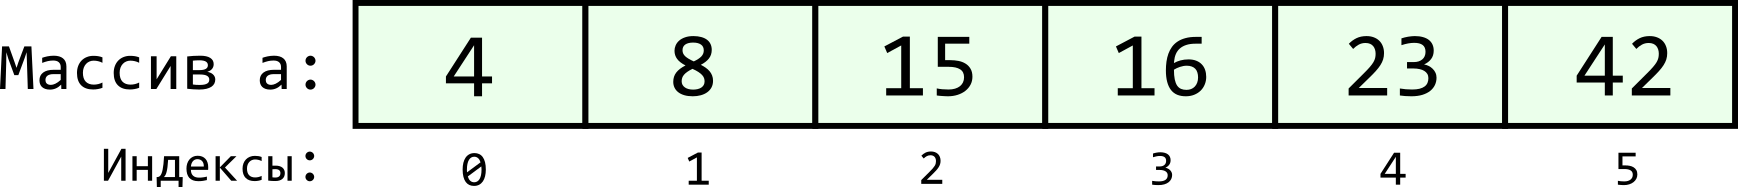
\includegraphics[scale=0.8]{../images/array_indexes.png}
\end{center}
Доступ к элементу по индексу осуществляется через квадратные скобки. Например, если мы хотим поменять в массиве, определённом выше, число 15 на 20 нужно написать: \texttt{a[2] = 20;}


\subsection*{Инициализация массива}
Объявить и инициализировать массив можно несколькими разными способами:
\begin{itemize}
\item Без инициализации. Такой массив обязательно нужно будет инициализировать в дальнейшем.
\begin{lstlisting}
int a[5]; 
\end{lstlisting}

\item Полная инициализация. Задаём все элементы.
\begin{lstlisting}
int a[5] = {1, 2, 3, 4, 5};
\end{lstlisting}

\item Неполная инициализация. В данном примере, мы задаём два элемента, а остальные автоматически занулятся. В результате массив \texttt{a} будет содержать следующие элементы: \texttt{1, 2, 0, 0, 0}. 
\begin{lstlisting}
int a[5] = {1, 2};
\end{lstlisting}

\item Инициализация нулями. Все элементы занулятся. Частный случай неполной инициализации.
\begin{lstlisting}
int a[10] = {0};
\end{lstlisting}

\item Автоматическое определение размера, если он не указан. Размер этого массива будет равен пяти.
\begin{lstlisting}
int a[] = {1, 2, 3, 4, 5};
\end{lstlisting}
\end{itemize}

\subsection*{Границы массива}
Выходить за границы массива опасно. Любой доступ за границы массива является очень грубой ошибкой -- неопределённым поведением.
\begin{lstlisting}
#include <stdio.h>
int main()
{
	int a[5] = {10, 20, 30, 40, 50};
	
	printf("%i\n", a[2]); 	// ОК, напечатает 30
	
	printf("%i\n", a[7]); 	// Грубая ошибка - неопределённое поведение.
	printf("%i\n", a[-2]); 	// Грубая ошибка - неопределённое поведение.
}
\end{lstlisting}
Наличие неопределённого поведения делает всё программу невалидной. При этом программа на вашем компьютере может не выдавать никаких сообщений об ошибке и даже делать что-то адекватное. Но это не значит, что ошибки в программе нет. Из-за того, что в программе присутствует неопределённое поведение, ошибки могут возникнуть на других системах или даже на вашей системе при следующем запуске. 

\subsection*{Печать массива на экран}
К сожалению в языке C нет стандартного способа распечатать массив на экран одной командой.
Один вызов функции \texttt{printf} также не может распечатать весь массив сразу.
Поэтому единственный вариант напечатать массив, это просто просто напечатать все его элементы, используя цикл, как это сделано в следующей программе:
\begin{lstlisting}
#include <stdio.h>
int main()
{
    int a[5] = {10, 20, 30, 40, 50};

    for (int i = 0; i < 5; ++i)
        printf("%i ", a[i]);
    printf("\n");
}
\end{lstlisting}

\subsection*{Присваивание массива}
К сожалению в языке C нет стандартного способа присваивания одного массива другому. Для присваивания также не работает синтаксис с фигурными скобочками, который работает для инициализации при объявлении. Поэтому единственный способ присвоить один массив другому -- это поэлементное присваивание в цикле.
\begin{lstlisting}
#include <stdio.h>
int main()
{
    int a[5] = {10, 20, 30, 40, 50};
    int b[5] = {90, 80, 70, 60, 50};

	//~ Ошибка, нельзя присваивать один массив другому
	a = b;	
	
	//~	Ошибка, фигурные скобки для задания массива работают только при объявлении			
    a = {11, 12, 13, 14, 15};	
    
    //~ Единственный способ:
    for (int i = 0; i < 5; ++i)
    	a[i] = b[i];
}
\end{lstlisting}

\subsection*{Считывание массива с экрана}
Также как и для печати, в языке C нет одной стандартной функции, которая бы считывала весь массив сразу.
Поэтому считывать нужно каждый элемент массива по отдельности в цикле. Пример программы, которая считывает 5 элементов и записывает из в массив, а затем печатает эти элементы, увеличенные на 1:
\begin{lstlisting}
#include <stdio.h>
int main()
{
    int a[5];
    for (int i = 0; i < 5; ++i)
        scanf("%i", &a[i]);

    for (int i = 0; i < 5; ++i)
        printf("%i ", a[i] + 1);
    printf("\n");
}
\end{lstlisting}


\subsection*{Считывание $n$ чисел с экрана в массив}


\newpage
\subsection*{Подмассивы}
Подмассив - это некоторая последовательная часть массива. В языке C нет никаких специальных средств для работы с подмассивами. Мы будем задавать подмассив в коде как два числа -- индексы граничных элементов. Будем обозначать подмассивом \texttt{a[l, r]} такую часть массива, элементы которого имеют индекс \texttt{i} в диапазоне \\
\texttt{l <= i < r}. Обратите внимание, что мы договорились, что элемент \texttt{a[r]} не входит в подмассив \texttt{a[l, r]}.\\

Например, в подмассив \texttt{[1, 4]} массива \texttt{a} входят элементы \texttt{8, 15, 16}, а элемент \texttt{23} не входит.
\begin{center}
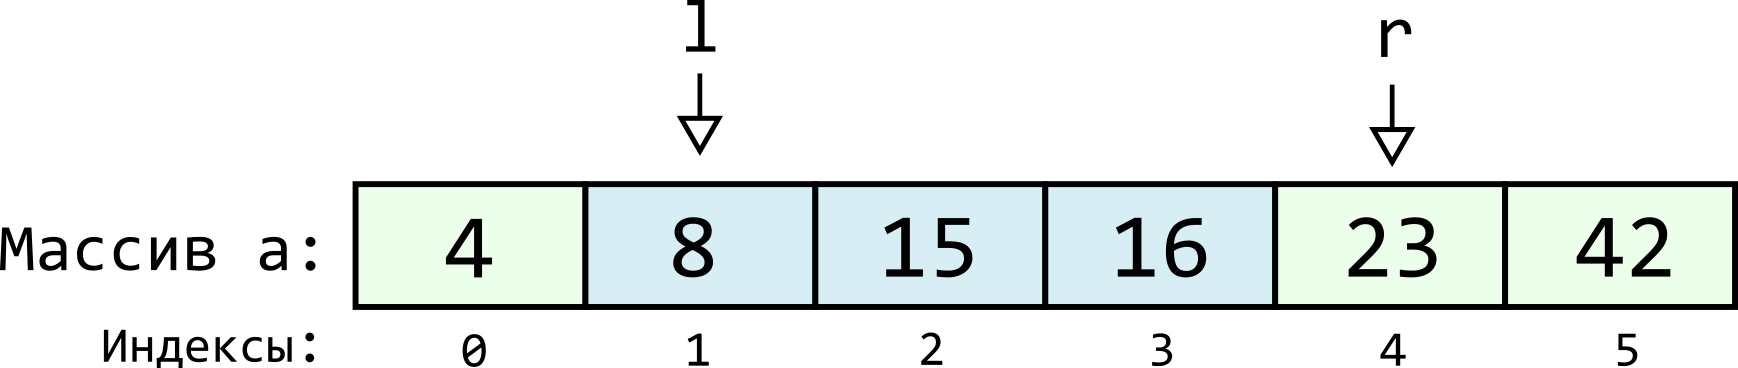
\includegraphics[scale=0.8]{../images/array_slice.png}
\end{center}


\subsection*{Сортировка}
Сортировка -- это упорядочение элементов по возрастанию, убыванию или по какому-то другому критерию.

\subsubsection*{Сортировка выбором} 
Сортировка выбором -- это простейший алгоритм сортировки, который заключается в следующем: \\
Для каждого подмассива \texttt{[j, n]} (где \texttt{j} последовательно меняется от \texttt{0} до \texttt{n - 1}) поменять местами первый и минимальный элементы этого подмассива. 


\begin{lstlisting}
for (int j = 0; j < n; ++j)
{
    int min_index = j;
    for (int i = j + 1; i < n; ++i)
    {
        if (a[i] < a[min_index])
            min_index = i;
    }

    int temp = a[j];
    a[j] = a[min_index];
    a[min_index] = temp;
}
\end{lstlisting}

\subsubsection*{Сортировка пузырьком} 
Сортировка пузырьком -- это простейший алгоритм сортировки, который заключается в следующем: \\
Для каждого подмассива \texttt{[0, n - j]} (где \texttt{j} последовательно меняется от \texttt{0} до \texttt{n - 1}) мы делаем следующую операцию: пробегаем по этому подмассиву и, если соседние элементы стоят неправильно, то меняем их местами.


\begin{lstlisting}
for (int j = 0; j < n; ++j)
{
    for (int i = 0; i < n - 1 - j; i += 1)
    {
        if (a[i] > a[i + 1])
        {
            int temp = a[i];
            a[i] = a[i + 1];
            a[i + 1] = temp;
        }
    }
}
\end{lstlisting}


\subsection*{Бинарный поиск на отсортированном массиве}
Если известно, что массив уже отсортирован, то многие задачи на таком массиве можно решить гораздо проще и/или эффективней. Например, просто найти минимум, максимум и медианное значение. Одной из задач, которая быстрее решается на отсортированном массиве -- это задача поиска элемента в массиве. Если массив отсортирован, то решить эту задачу можно гораздо быстрее чем простой обход всех элементов. \\

Предположим, что массив отсортирован по возрастанию и надо найти элемент \texttt{x} в этом массиве или понять, что такого элемента в массиве не существует. Для этого мы мысленно разделим массив на  2 части:
\begin{enumerate}
\item Элементы, которые меньше, чем \texttt{x}
\item Элементы, которые больше или равны \texttt{x}
\end{enumerate}

Затем введём две переменные-индекса \texttt{l} и \texttt{r}. В начале работы алгоритма индекс \texttt{l} будет хранить индекс фиктивного элемента, находящегося до первого (то есть \texttt{l = -1}), а индекс \texttt{r} будет хранить индекс фиктивного элемента, находящимся после последнего (то есть \texttt{r = n}). 

На каждом шаге алгоритма мы будем брать середину между индексами \texttt{l} и \texttt{r} и передвигать к этой середине или индекс \texttt{l} или индекс \texttt{r}. При этом при изменении индексов должны соблюдаться условия:
\begin{verbatim}
a[l] < x
a[r] >= x
\end{verbatim}

Алгоритм закончится тогда, когда разница между индексами не станет равным 1, то есть не станет \\
\texttt{r == l + 1}. И так как \texttt{a[l] < x} и \texttt{a[r] >= x}, то если элемент \texttt{x} в массиве существует, то его индекс равен \texttt{r}.



Код для поиска в отсортированном массиве бинарным поиском:
\begin{lstlisting}
#include <stdio.h>

int main() 
{
    int n;
    int a[1000];
    scanf("%i", &n);
    for (int i = 0; i < n; ++i)
        scanf("%i", &a[i]);
        
    int x;
    scanf("%i", &x);
    
    int l = -1, r = n;
    while (r > l + 1) 
    {
        int mid = (l + r) / 2;
        
        if (a[mid] >= x)
            r = mid;
        else 
            l = mid;
    }
    
    if (r < n && a[r] == x)
        printf("Element found! Index = %i\n", r);
    else
        printf("Element not found!");
}

\end{lstlisting}


\section*{Дополнительный материал}
\subsection*{Объявление несколько переменных в одной строке}
\subsection*{Возвращаемое значение функции \texttt{printf}}
\subsection*{Возвращаемое значение функции \texttt{scanf}}
\subsection*{Считывание последовательности чисел неизвестной длины}

\subsection*{Независимость потоков \texttt{stdin} и \texttt{stdout}}

\subsection*{Буферизация \texttt{scanf}}

\subsection*{Особенность логических операторов}
\subsection*{Тернарный оператор}
\subsection*{Оператор запятая}

\end{document}